\documentclass[12pt,letterpaper]{article}
\usepackage[utf8]{inputenc}
\usepackage[spanish]{babel}
\usepackage{graphicx}
\usepackage[left=2cm,right=2cm,top=2cm,bottom=2cm]{geometry}
\usepackage{graphicx} % figuras
% \usepackage{subfigure} % subfiguras
\usepackage{float} % para usar [H]
\usepackage{amsmath}
%\usepackage{txfonts}
\usepackage{stackrel} 
\usepackage{multirow}
\usepackage{enumerate} % enumerados
\renewcommand{\labelitemi}{$-$}
\renewcommand{\labelitemii}{$\cdot$}
% \author{}
% \title{Caratula}
\begin{document}

% Fancy Header and Footer
% \usepackage{fancyhdr}
% \pagestyle{fancy}
% \cfoot{}
% \rfoot{\thepage}
%

% \usepackage[hidelinks]{hyperref} % CREA HYPERVINCULOS EN INDICE

% \author{}
\title{Caratula}

\begin{titlepage}
\begin{center}
\large{UNIVERSIDAD PRIVADA-DE-TACNA}\\
\vspace*{-0.025in}
\begin{figure}[htb]
\begin{center}

\includegraphics[width=8cm]{./Imagenes/logo}
\end{center}
\end{figure}
\vspace*{0.15in}
INGENIERIA DE SISTEMAS  \\

\vspace*{0.5in}
\begin{large}
TITULO:\\
\end{large}

\vspace*{0.1in}
\begin{Large}
\textbf{TRABAJO FINAL DE UNIDAD I} \\
\end{Large}

\vspace*{0.3in}
\begin{Large}
\textbf{CURSO:} \\
\end{Large}

\vspace*{0.1in}
\begin{large}
INTELIGENCIA DE NEGOCIOS\\
\end{large}

\vspace*{0.3in}
\begin{Large}
\textbf{DOCENTE(ING):} \\
\end{Large}

\vspace*{0.1in}
\begin{large}
 Patrick Cuadros Quiroga\\
\end{large}

\vspace*{0.2in}
\vspace*{0.1in}
\begin{large}
Integrantes: \\
\begin{flushleft}

Andrés de la Barra Vásquez            	\hfill	(2016055087) \\
David Damian Mamani 			\hfill	(2016055194) \\
Andre Reinoso Aranda 			\hfill	(2016055275) \\
Samuel Nuñez Mamani 			\hfill	(2016054462) \\

\end{flushleft}
\end{large}
\end{center}

\end{titlepage}


\tableofcontents % INDICE
\thispagestyle{empty} % INDICE SIN NUMERO
\newpage
\setcounter{page}{1} % REINICIAR CONTADOR DE PAGINAS DESPUES DEL INDICE

%%------------------------------------------------------------------------------------
\begin{abstract}

El presente trabajo desea plantear de forma breve y concisa la utilización del chatbot, desarrollado con las herramientas proporcionadas por Azure y el convenio con la universidad, siendo su prioridad la agilización de datos ya sea de los docentes, eventos o hasta los números de teléfonos de una escuela.


\begin{center}
\textbf{Abstract}
\end{center}
The present work wishes to briefly and concisely discuss the use of chatbot, developed with the tools provided by Azure and the agreement with the university, with the priority being the streamlining of data from teachers, events or even the telephone numbers of a school.

\end{abstract}
\newpage
\section{INTRODUCCION}
El servicio de tutoría, o de cada escuela de la facultad puede brindar información necesaria ya sea para los próximos eventos, teléfonos, email de los docentes, etc. si se acude a ellas en consulta por algún tema. 
Otro modo de trabajo para la tutoría es usar los medios sociales, ya que hace más fácil el trabajo mientras que ya es posible responder a las preguntas de los estudiantes de forma remota. 
Pero a veces el sistema se vuelve ineficaz por la falta de disponibilidad, o sea que el horario no es de ayuda para algunos interesados, o que simplemente no se hace posible la trata de muchas personas al mismo tiempo.
Un chatbot es necesario para tener el servicio de información la mayor cantidad del tiempo posible haciendo que tutoría se centre en otro tipo de asuntos de mayor importancia y envergadura. 




\newpage
%---------------------------------------------
\section{TITULO}
	\par Chatbot
\section{AUTORES}

\begin{itemize}
	\item De la Barra Vásquez, Andrés Eduardo
	\item Reinoso Aranda, Andre Sebastian
	\item Damian Mamani, David
	\item Nuñez Mamani, Samuel
	
\end{itemize}

%---------------------------------------------


%---------------------------------------------
\section{PLANTEAMIENTO DEL PROBLEMA}
	\subsection{Problema}
El servicio de tutoría, o de cada escuela de la facultad puede brindar información si se acude a ellas en consulta por algún tema. Otro modo de trabajo para la tutoría es usar los medios sociales, ya que hace más fácil el trabajo mientras que ya es posible responder a las preguntas de los estudiantes de forma remota. Pero a veces el sistema se vuelve ineficaz por la falta de disponibilidad, o sea que el horario no es de ayuda para algunos interesados, o que simplemente no se hace posible la trata de muchas personas al mismo tiempo.\\
	\subsection{Justificación}
El presente proyecto busca hacer mucho más fácil y rápida la comunicación con un agente de la escuela para la toma de datos e información básica que la pida el estudiante. De este modo, el agente puede reemplazar o hacer de apoyo para cuando la escuela no esté disponible.
	\subsection{Alcance}
Se espera que el sistema pueda ser operado por todos los estudiantes, y consultado desde su Smartphone.

%---------------------------------------------
\section{OBJETIVOS}
	\subsection{General}
\begin{itemize}
	\item Construir un sistema que esté en la capacidad de responder a diferentes dudas y preguntas que presenten los estudiantes, con la finalidad de agilizar el trabajo de respuesta de cada escuela en la facultad de ingeniería.
\end{itemize}

	\subsection{Específicos}
\begin{itemize}
	\item Crear un sistema inteligente con información básica acerca de la escuela como de docentes, cursos, eventos, teléfonos, temas, etc.
	\item Ofrecer una interfaz interactiva para la gestión de la información que se pretende brindar.
	\item Asegurar un servicio que esté disponible las 24 horas de su uso a través del servicio que nos brinda Azure y el convenio con la Universidad.
\end{itemize}



%---------------------------------------------
\section{REFERENTES TEÓRICOS}
\begin{itemize}
	\item \textbf{¿Qué es un chatbot?} \\ 
Un chatbot es una tecnología que permite al usuario mantener una conversación a través de un software que se integra en un determinado sistema de mensajería, como, por ejemplo: Facebook, Twitter, Telegram, Whatsapp, etc. El sistema está programado para que interactúe con el cliente y le resuelva dudas, pero sin que haya una persona física contestando. Tienen la ventaja de que están disponibles siempre para resolver las dudas de los usuarios que quieran contactar contigo a cualquier hora del día.

	\item \textbf{Tipos de ChatBot}\\
	\textbf{Dumb ChatBots}\\ 
ChatBot mas comun en el mercado. Se definen siguiendo unas reglas preestablecidas, protocolos o patrones, funcionan de manera independiente.Se programan siguiendo esta estructura:
\\
-Usuario pregunta algo.\\
-En base a ello, el bot contesta esto.\\


	\textbf{Smart ChatBots}\\
Este tipos de ChatBots que son mucho más inteligentes que los anteriores, más interactivos, acercándose a la forma de reaccionar del ser humano en lenguaje Natural. Mantener una conversación más fluida y lógica de la que podríamos tener con un contestador automático.

Para funcionar, procesan el lenguaje, pudiendo entender la petición que el cliente pueda tener y reaccionar ante la misma. Además, también interpretan las diferentes interpretaciones.

Una de las principales características de este tipo de Chatbot es que es capaz de aprender ante cada conversación (Machine Learning).


	\item  \textbf{¿Qué es un Sistema de Recomendaciones?} \\
Es un sistema inteligente que proporciona a los usuarios una serie de sugerencias personalizadas (recomendaciones) sobre un determinado tipo de elementos (items). Los sistemas de recomendación estudian las características de cada usuario y mediante un procesamiento de los datos, encuentra un subconjunto de items que pueden resultar de interés para el usuario.


\end{itemize}

%---------------------------------------------
\section{DESARROLLO DE LA PROPUESTA}
	\subsection{Tecnología de información}
	\begin{itemize}
	\item \textbf{Microsoft Azure} \\ 
	\item \textbf{Base de datos Sql Server} \\ 
\item \textbf{NetBeans 8.1} \\ 
\item \textbf{JDK 1.8} \\ 


\end{itemize}
	\subsection{Metodología, técnicas usadas}
 \begin{itemize}
	\item \textbf{Scrum} \\ 

\end{itemize}
%---------------------------------------------
\section{CRONOGRAMA}

\begin{center}
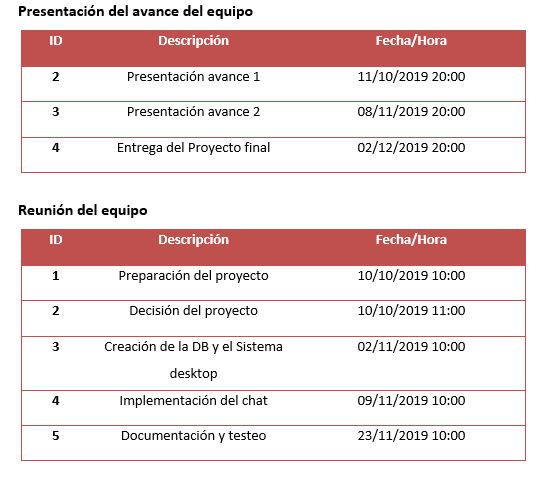
\includegraphics[width=0.8\textwidth]{./Imagenes/cronograma}

\end{center}

%---------------------------------------------------------------------------------------
\cite{1}
\bibliographystyle{plain}
\bibliography{Bibliografia}

\end{document}
